\documentclass{../industrial-development}
\graphicspath{{07-version-control-system/}}

\title{Использование систем управления версиями в промышленной разработке}
\author{Заплатин Егор Сергеевич, ПИ-21 МО}
\date{}

\begin{document}

\begin{frame}
  \titlepage
\end{frame}

\begin{frame}{План лекции}
  \tableofcontents
\end{frame}

\section{Введение}

\subsection{Что такое система управления версиями}

\begin{frame} \frametitle{Что такое система управления версиями}
  \begin{block}{Определение}
    \alert{Системы контроля версий} --- это категория программных инструментов, которые помогают команде программного обеспечения управлять изменениями исходного кода с течением времени
  \end{block}
  
  \begin{itemize}
  \item Каждая модификация кода отслеживается в специальном виде в базе данных
  \item При обнаружении ошибки можно вернуться к прошлому коду, сравнить исходный код с предыдущими версиями
  \end{itemize}
\end{frame}

\lecturenotes

Контроль версий помогает отслеживать каждое индивидуальное изменение каждым вкладчиком, помогает предотвратить конфликты при параллельной работе. Изменения, внесенные в одну часть программного обеспечения, могут быть несовместимы с изменениями, внесенными другим разработчиком, работающим параллельно. Эта проблема должна быть обнаружена и решена упорядоченным образом, не блокируя работу остальной команды. Кроме того, во всех разработках программного обеспечения любое изменение может вводить новые ошибки, и новому коду нельзя доверять, пока он не будет протестирован. Поэтому тестирование и разработка продолжаются до тех пор, пока не будет готова новая версия~\cite{Atlassian}.

\subsection{Преимущества систем контроля версий}

\begin{frame} \frametitle{Преимущества систем контроля версий}

  \begin{itemize}
  \item Полная долгосрочная история изменений каждого файла
  \item Ветвление и слияние
  \item Отслеживаемость
  \end{itemize}
\end{frame}

\begin{frame} \frametitle{Полная долгосрочная история изменений каждого файла}

  \begin{itemize}
  \item Сохранются все изменения каждого файла, сделанные многими людьми на протяжении долгих лет
  \item Каждое изменение включает в себя автора, дату и письменные заметки о целях изменения
  \item Каждое изменение изменет свой номер --- версию (ревизию)
  \end{itemize}
\end{frame}

\lecturenotes

Имеются ввиду все изменения, сделанные многими людьми на протяжении многих лет. Изменения включают в себя создание и удаление файлов, а также редактирование их содержимого. Различные инструменты VCS отличаются тем, насколько хорошо они могут обрабатывать переименование и перемещение файлов. Эта история должна также включать автора, дату и письменные заметки о целях каждого изменения. Наличие полной истории позволяет вернуться к предыдущим версиям, помогает в анализе причин ошибок, и это важно, когда нужно исправлять проблемы в более старых версиях программного обеспечения. Если программное обеспечение активно разрабатывается, почти все можно считать «более старой версией» программного обеспечения~\cite{Atlassian}.

\begin{frame} \frametitle{Ветвление и слияние}
  
  \begin{itemize}
  \item Возможность создания веток позволяет нескольким разработчикам работать над одним проектом независимо друг от друга
  \item Ветки можно объединять воедино, сливая сделанные изменения
  \item Предоставляется интерфейс для разрешения конфликтов при слиянии
  \end{itemize}
\end{frame}

\lecturenotes

Наличие членов команды работающих параллельно не простая ситуация, но даже люди, работающие самостоятельно, могут извлечь выгоду из способности работать над независимыми потоками изменений. Создание «ветки» в инструментах VCS позволяет нескольким потокам работать независимо друг от друга, а также предоставляет возможность объединить эту работу вместе, позволяя разработчикам проверять, что изменения в каждой ветке не конфликтуют. Многие команды программного обеспечения применяют практику ветвления для каждой функции или ветвления для каждой версии, или и то, и другое. Существует множество различных рабочих процессов, которые команды могут выбирать, когда они решают, как использовать ветвление и объединяющие объектов в VCS~\cite{Atlassian}.

\begin{frame} \frametitle{Пример ветвления}
  \centerline{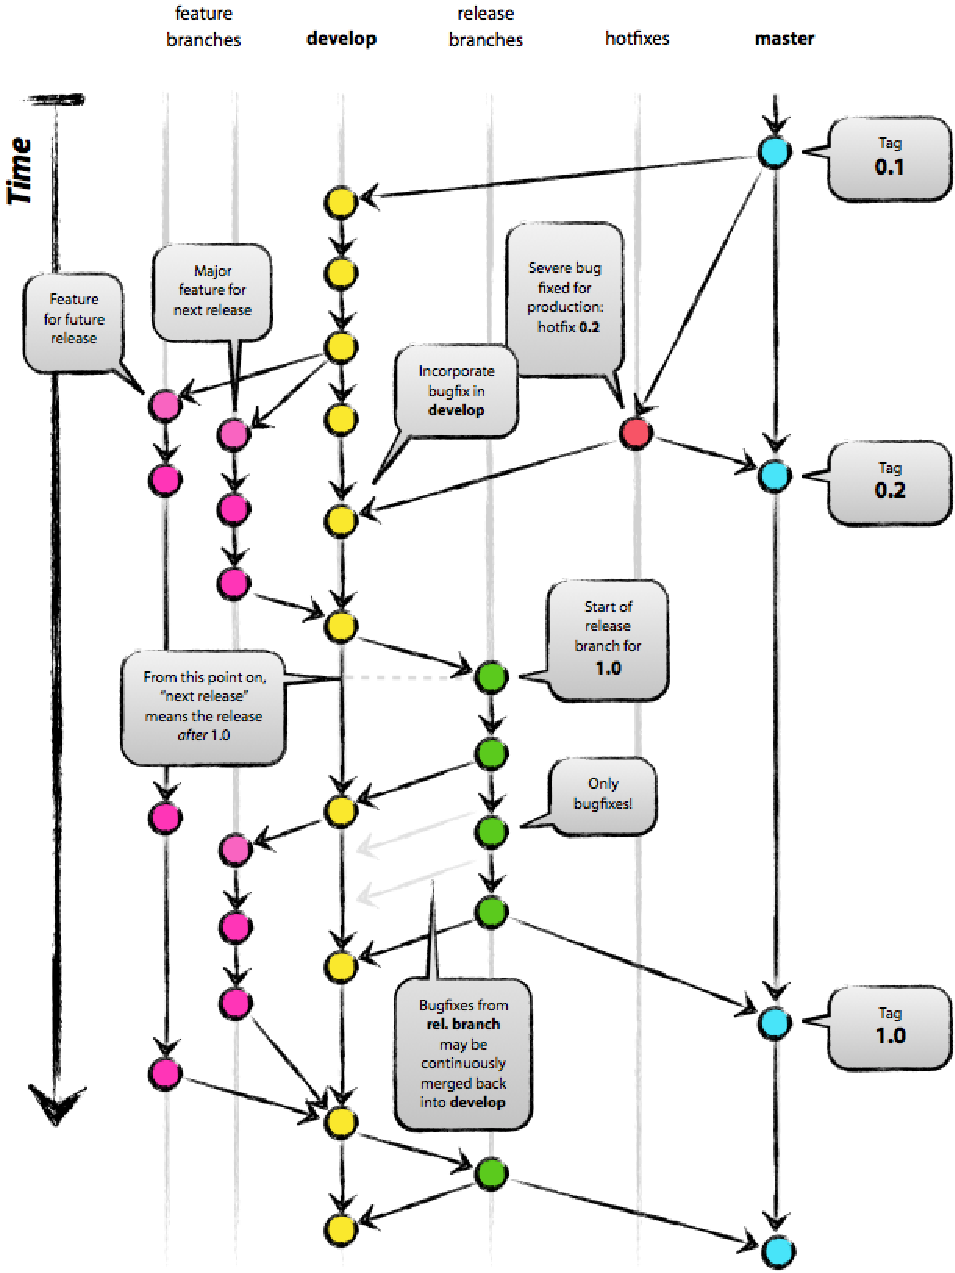
\includegraphics[width=0.5\textwidth]{branching.pdf}}
\end{frame}

\begin{frame} \frametitle{Отслеживаемость}
 
  \begin{itemize}
  \item Всегда можно понять когда и зачем код был написан
  \item Легко проводить анализ причинно-следственных связей
  \end{itemize}
\end{frame}

\lecturenotes

Возможность отслеживать каждое изменение, внесенное в программное обеспечение, и подключать его к программам управления проектами и программам отслеживания ошибок, таким как Jira, возможность комментировать каждое изменение сообщением, описывающим цель и намерение изменения, может помочь не только при анализе причинно-следственных связей и других экспертиз. Имея под рукой аннотированную историю кода, можно прочитать код, пытаясь понять, что он делает и почему он так сконструирован. Это может позволяет разработчикам делать правильные и гармоничные изменения, соответствующие намеченному долгосрочному дизайну системы. Это может быть особенно важно для эффективной работы с устаревшим кодом и имеет решающее значение для того, чтобы разработчики могли оценивать будущую работу с любой точностью~\cite{Atlassian}.

\section{Виды систем контроля версий}

\subsection{Централизованные системы контроля версий}

\begin{frame} \frametitle{Централизованные системы контроля версий}
  \begin{block}{Определение}
    В \alert{централизованных системах контроля версий} есть центральный сервер, на котором хранятся все файлы под версионным контролем, и ряд клиентов, которые получают копии файлов 
из него
  \end{block}
 
\end{frame}

\begin{frame} \frametitle{Схема централизованного контроля версий}
  \centerline{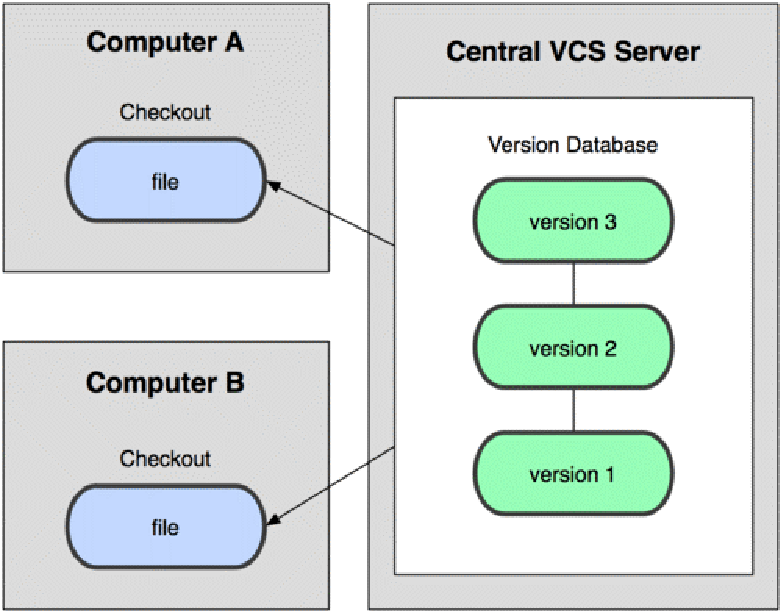
\includegraphics[width=0.7\textwidth]{centralizedVCS.pdf}}
\end{frame}

\begin{frame} \frametitle{Особенности централизованных систем контроля версий}
  \begin{itemize}
  \item Удобное администрирование: администраторы имеют четкий контроль над тем, кто и что может делать
  \item Центральный сервер является уязвимым местом всей системы, при его повреждении можно потерять всю историю проекта
  \end{itemize}
\end{frame}

\lecturenotes

Такой подход имеет множество преимуществ. К примеру, все знают, кто и чем занимается в проекте. У администраторов есть чёткий контроль над тем, кто и что может делать, и, конечно, администрировать ЦСКВ намного легче, чем локальные базы на каждом клиенте.

Однако при таком подходе есть и несколько серьёзных недостатков. Наиболее очевидный — централизованный сервер является уязвимым местом всей системы. Если сервер выключается на час, то в течение часа разработчики не могут взаимодействовать, и никто не может сохранить новой версии своей работы. Если же повреждается диск с центральной базой данных и нет резервной копии, вы теряете абсолютно всё — всю историю проекта, разве что за исключением нескольких рабочих версий, сохранившихся на рабочих машинах пользователей~\cite[с.~6--7]{ProGit}.

\subsection{Распределённые системы контроля версий}

\begin{frame} \frametitle{Распределённые системы контроля версий}
  \begin{block}{Определение}
    В \alert{распределённых системах контроля версий} клиенты не просто выгружают последние версии файлов, а полностью копируют весь репозиторий. Каждый раз, когда клиент забирает свежую версию файлов, он создаёт себе полную копию всех данных
  \end{block}
 
\end{frame}

\begin{frame} \frametitle{Схема распределённой системы контроля версий}
  \centerline{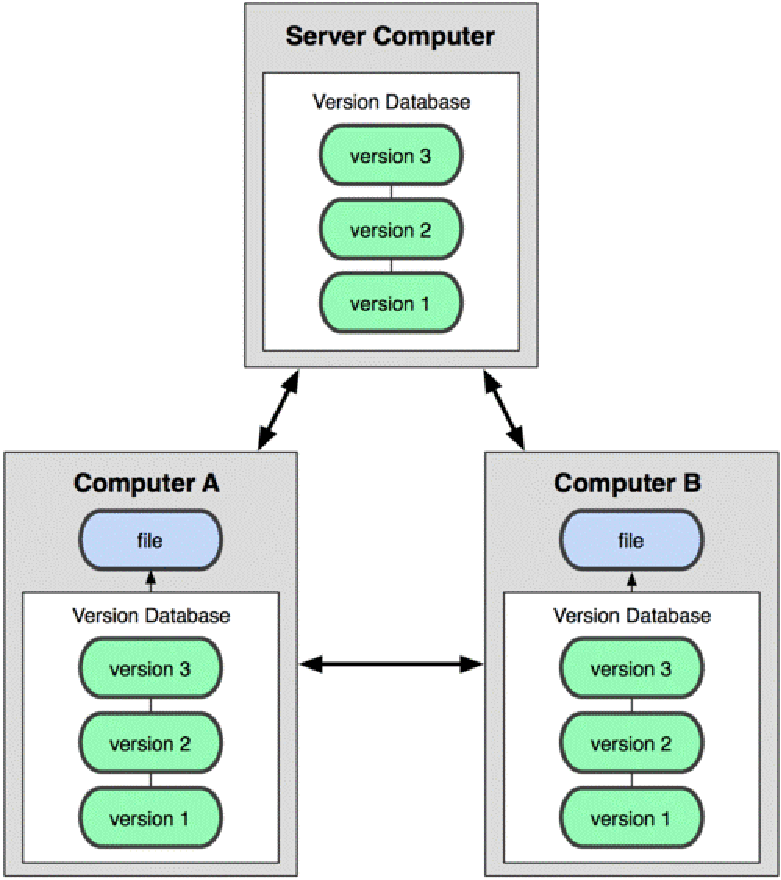
\includegraphics[width=0.5\textwidth]{distributedVCS.pdf}}
\end{frame}

\begin{frame} \frametitle{Особенности распределённых систем контроля версий}
  \begin{itemize}
  \item При повреждении удалённого сервера любой клиент может полностью восстановить базу данных
  \item Можно работать с несколькими удалёнными репозиториями, одновременно вести несколько типов рабочих процессов
  \end{itemize}
\end{frame}

\lecturenotes

В случае, когда «умирает» сервер, через который шла работа, любой клиентский репозиторий может быть скопирован обратно на сервер, чтобы восстановить базу данных. 

Кроме того, в большей части этих систем можно работать с несколькими удалёнными репозиториями, таким образом, можно одновременно работать по-разному с разными группами людей в рамках одного проекта. Так, в одном проекте можно одновременно вести несколько типов рабочих процессов, что невозможно в централизованных системах~\cite[с.~7]{ProGit}.

\section{Популярные системы контроля версий}

\subsection{Subversion}

\begin{frame} \frametitle{Subversion}
  \begin{block}{}
    \alert{Subversion (также известная как «SVN»)} --- свободная централизованная система управления версиями, официально выпущенная в 2004 году компанией CollabNet. С 2010 года Subversion является одним из проектов Apache Software Foundation и официально называется Apache Subversion
  \end{block}
\end{frame}

\begin{frame} \frametitle{Ревизии в SVN}
  
  \begin{itemize}
  \item Номер ревизии --- это натуральное число (начиная с нуля)
  \item Каждая успешная фиксация изменений пораждает ровно одну новую ревизию в хранилище
  \item Ревизия характеризует состояние не отдельного файла, а всего хранилища в целом
  \end{itemize}
\end{frame}

\lecturenotes

Номера ревизий

Номер ревизии в Subversion — это натуральное число (или 0 для самой первой ревизии), адресующее номер состояния хранилища в процессе изменения содержащихся в нём данных. Каждая успешная фиксация изменений порождает ровно одну новую ревизию в хранилище, то есть N-я ревизия — это состояние хранилища после N-й фиксации.

В Subversion ревизия характеризует состояние не отдельного файла, а всего хранилища в целом. Например, ревизия 32 — это состояние четырёх файлов и двух директорий, существовавших в хранилище на тот момент.

Номер ревизии является аналогом времени в том смысле, что меньшие номера ревизий соответствуют более ранним состояниям хранилища, а бо́льшие — поздним.

Минимальный номер ревизии 0 (ноль) соответствует изначальному состоянию хранилища, когда ещё не было зафиксировано ни одной правки. В нулевой ревизии хранилище содержит только пустую корневую директорию.
Максимальный номер ревизии соответствует самому последнему состоянию хранилища, то есть состоянию после фиксации последней правки. Вместо указания номера последней ревизии можно использовать ключевое слово HEAD (головная ревизия); это удобно, поскольку номер головной ревизии увеличивается при каждой фиксации изменений.

Номер ревизии можно рассматривать как некую временну́ю отметку в истории хранилища. Более того, с каждым номером ревизии связано абсолютное значение времени, когда эта ревизия была сделана (свойство svn:date). Однако указание номера ревизии удобнее, чем указание времени, так как нет путаницы с часовыми поясами, запись номера короче и номер ревизии не может быть изменён~\cite{SVNWikipedia}.

\begin{frame} \frametitle{Ветвление в SVN}
  
  \begin{itemize}
  \item Subversion использует «файловую» модель для реализации ветвей, то есть ветвь является обычной директорией
  \item Ветка --- это копия директории svn, содержащая только изменения, одинаковые файлы не копируются (создаются ссылки на них)
  \item Так же используется метки, создание метки технически не отличается от создания ветви, но предполагается, что никто не будет изменять данные в метке
  \end{itemize}
\end{frame}

\lecturenotes

Метки

Создание метки также производится командой svn copy, то есть технически не отличается от создания ветви. Отличие только в способе использования: предполагается, что никто не будет изменять данные в метке (фиксировать в неё изменения).

Концепция меток, используемая в Subversion, отличается от концепции меток в других системах управления версиями. Обычно метка является символическим именем, которое адресует набор файлов и их состояние. В Subversion метка копирует набор файлов и их состояние. Метки-копии в Subversion имеют свои достоинства и недостатки.

Достоинства:

    метка видна в структуре директорий, можно сделать удобную древовидную организацию меток.

Недостатки:

    трудно узнать, в какие метки вошёл файл (то же для директории);
    если права доступа установлены индивидуально для директорий, то метка эти права не наследует;
    содержимое метки может быть изменено;
    если из метки создать рабочую копию и зафиксировать из этой рабочей копии какие-либо изменения, то это изменит саму метку, а не те данные, которые были помечены. Правильным способом работы «от метки» является создание рабочей копии не из метки, а из того, что является источником этой метки~\cite{SVNWikipedia}.


\begin{frame} \frametitle{Пример ветвления}
  \centerline{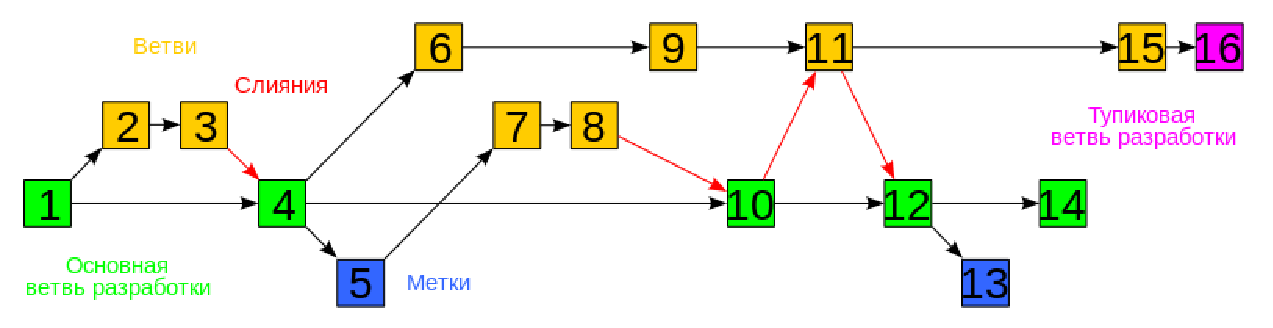
\includegraphics[width=0.9\textwidth]{branching-svn.pdf}}
\end{frame}

\begin{frame} \frametitle{Основные возможности Subversion}
  
  \begin{itemize}
  \item Контроль изменений каталогов
  \item Каждый набор изменений либо попадает в хранилище целиком, либо не попадает туда вовсе
  \item Возможность конкурентной многопользовательской работы с хранилищем
  \item Каждый файл и каталог имеет собственный набор свойств, представленных в виде названия и значения
  \item Subversion обнаруживает различия между файлами с помощью специального бинарного алгоритма, который одинаково работает как с текстовыми, так и с бинарными файлами
  \item Subversion создаёт ветки и метки путём простого копирования проекта, используя механизм, похожий на жёсткие ссылки в файловых системах
  \end{itemize}
\end{frame}

\lecturenotes

Subversion предоставляет следующие возможности:
Контроль изменений каталогов 
Subversion использует «виртуальную» файловую систему с возможностями управления версиями, которая способна отслеживать изменения во времени целых структур каталогов. Под управление версиями попадают и файлы, и каталоги.

Настоящая история версий 
Subversion делает возможным добавление, удаление, копирование и переименование как файлов, так и каталогов. При этом каждый вновь добавленный файл начинает жизнь с чистого листа, сохраняя собственную историю изменений.

Атомарная фиксация изменений 
Каждый набор изменений либо попадает в хранилище целиком, либо не попадает туда вовсе. Это позволяет разработчикам создавать и фиксировать изменения логически оправданными кусками, предотвращая тем самым проблемы, которые могут возникать в тех случаях, когда только часть необходимых изменений помещается в хранилище успешно.

Возможность конкурентной многопользовательской работы с хранилищем
Поддержка конкурентной (в том числе одновременной, с изоляцией транзакций) многопользовательской работы с хранилищем и, в большинстве случаев, автоматическим слиянием изменений различных разработчиков (в рабочей копии);

Метаданные с версиями 
Каждый файл и каталог имеет собственный набор свойств, представленных в виде названия и значения. Вы можете создавать и сохранять любые необходимые пары названий свойств и их значений. Свойства файлов точно так же находятся под управлением версиями, как и их содержимое.

Единый способ работы с данными 
Subversion обнаруживает различия между файлами с помощью специального бинарного алгоритма, который одинаково работает как с текстовыми, так и с бинарными файлами. Файлы записываются в хранилище в сжатом виде независимо от их типа, а различия между отдельными версиями могут передаваться по сети в обоих направлениях.

Эффективные ветки и метки 
Плата за использование веток и меток не должна быть пропорциональна размеру проекта. Subversion создаёт ветки и метки путём простого копирования проекта, используя механизм, похожий на жёсткие ссылки в файловых системах. Благодаря этому, операции по созданию веток и меток занимают немного времени~\cite[с.~14--15]{VSwithSVN}.

\begin{frame} \frametitle{Дополнительные возможности Subversion}
  
  \begin{itemize}
  \item Различные варианты доступа к хранилищу (непосредственный доступ на диске, по собственному сетевому протоколу или через веб-сервер по протоколу WebDAV/DeltaV)
  \item Возможность зеркалирования хранилища
  \item Два возможных внутренних формата хранилища: база данных или набор обычных файлов
  \item Библиотеки для языков PHP, Python, Perl, Java позволяют встроить функциональность клиента Subversion в программы, написанные на этих языках
  \item Многоуровневая архитектура библиотек, изначально рассчитанная на клиент-серверную модель
  \end{itemize}
\end{frame}

\lecturenotes

Различные варианты доступа к хранилищу, в том числе, непосредственным доступом на диске, по собственному сетевому протоколу или через веб-сервер по протоколу WebDAV/DeltaV.
Возможность зеркалирования хранилища.
Два возможных внутренних формата хранилища: база данных или набор обычных файлов.
Библиотеки для языков PHP, Python, Perl, Java позволяют встроить функциональность клиента Subversion в программы, написанные на этих языках.
Многоуровневая архитектура библиотек, изначально рассчитанная на клиент-серверную модель~\cite{SVNMotu}.

\begin{frame} \frametitle{Недостатки Subversion}
  \begin{itemize}
  \item Subversion не всегда может правильно обработать операции переименования файлов, если одновременно с переименованием изменяется и содержимое файла
  \item Слабая поддержка слияния ветвей
  \item Невозможность удаления данных из хранилища
  \item Папка .svn в каждой папке
  \end{itemize}
\end{frame}

\lecturenotes

Проблемы при переименовании файлов
Subversion не всегда может правильно обработать операции переименования файлов, если одновременно с переименованием изменяется и содержимое файла. Проблемы могут также возникнуть, если файл, переименованный в локальной копии, кто-то другой изменил в хранилище. Часть этих проблем исправлена в версии 1.5, однако это решение пока не полное.

Слабая поддержка слияния ветвей
Также слабым местом Subversion считают операции слияния веток. До версии 1.5 все такие операции пользователям приходилось отслеживать вручную, с помощью подробных записей в журнале изменений. Начиная с версии 1.5 появилась базовая поддержка автоматического отслеживания слияний, которую разработчики планируют улучшить в последующих релизах. В настоящее время Subversion достаточно хорошо поддерживает типовые сценарии слияния; в более сложных случаях возможны проблемы. Рекомендуется организовать рабочий процесс так, чтобы избежать проблемных сценариев. Слияние переименованных файлов и директорий не поддерживается.

Невозможность удаления данных из хранилища
Информация, однажды помещённая в хранилище Subversion, остаётся там навсегда: файл можно удалить в текущей ревизии, но всегда есть возможность получить из хранилища одну из предыдущих ревизий, в которых файл существовал. Хотя сохранность прошлых ревизий и является, собственно, целью использования систем управления версиями, иногда бывает необходимо полностью удалить из хранилища информацию, попавшую туда по ошибке. В Subversion не предусмотрено для этого никакого штатного способа; единственная возможность заключается в создании дампа хранилища, его обработке штатной утилитой svndumpfilter и последующем восстановлении хранилища из дампа. Существуют также сторонние программы для автоматизации этого процесса, но, в любом случае, для выполнения этой операции требуется временное прекращение доступа к хранилищу и вмешательство администратора с привилегиями, достаточно высокими для того, чтобы полностью стереть старое хранилище и заменить его новым.

Папка .svn в каждой папке
засоряет файловую структуру проекта. Начиная с версии 1.7 в корне рабочей копии проекта создаётся одна директория .svn, метаданные в которой сохраняются с использованием SQLite~\cite{SVNWikipedia}.

\subsection{Git}

\begin{frame} \frametitle{Git}
  \begin{block}{}
    \alert{Git} --- распределённая система управления версиями. Проект был создан Линусом Торвальдсом для управления разработкой ядра Linux, первая версия выпущена 7 апреля 2005 года. На сегодняшний день его поддерживает Джунио Хамано
  \end{block}
\end{frame}

\begin{frame} \frametitle{Ревизии в Git}
  
  \begin{itemize}
  \item Номер ревизии --- это хэш коммита (функция sha1)
  \item При создании новой ревизии система запоминает, как выглядит каждый файл в этот момент, и сохраняет ссылку на этот снимок
  \item Если файлы не были изменены, Git не запоминает эти файлы вновь, а только создаёт ссылку на предыдущую версию идентичного файла, который уже сохранён
  \end{itemize}
\end{frame}

\lecturenotes

Основное отличие Git’а от любой другой СКВ, это подход Git’а к работе со своими данными. Концептуально, большинство других систем хранят информацию в виде списка изменений в файлах. Эти системы представляют информацию в виде набора файлов и изменений, сделанных в каждом файле, по времени. 
Git не хранит и не обрабатывает данные таким способом. Вместо этого, подход Git’а к хранению данных больше похож на набор снимков миниатюрной файловой системы. Каждый раз, когда вы делаете коммит, то есть сохраняете состояние своего проекта в Git’е, система запоминает, как выглядит каждый файл в этот момент, и сохраняет ссылку на этот снимок. Для увеличения эффективности, если файлы не были изменены, Git не запоминает эти файлы вновь, а только создаёт ссылку на предыдущую версию идентичного файла, который уже сохранён. Git представляет свои данные как, скажем, поток снимков.

Это очень важное отличие между Git и почти любой другой СКВ. Git переосмысливает практически все аспекты контроля версий, которые были скопированы из предыдущего поколения большинством других систем. Это делает Git больше похожим на миниатюрную файловую систему с удивительно мощными утилитами, надстроенными над ней, нежели просто на СКВ~\cite[с.~8]{ProGit}.

\begin{frame} \frametitle{Ветвление в Git}
  
  \begin{itemize}
  \item Ветка --- указатель на один из коммитов
  \item При создании ветки создается новый указатель для дальнейшего перемещения
  \item Git хранит специальный указатель HEAD, указывающий на текущую локальную ветку
  \item Операция создания ветки выполняется почти мгновенно, переключение между ветками, также быстро
  \end{itemize}
\end{frame}

\lecturenotes

О ветвлении в двух словах

Для четкого понимания механизма ветвлений, необходимо вернуться назад и изучить то, как Git хранит данные.

Как вы можете помнить из Введение, Git не хранит данные в виде последовательности изменений, он использует набор снимков (snapshot).

Когда вы делаете коммит, Git сохраняет его в виде объекта, который содержит указатель на снимок (snapshot) подготовленных данных. Этот объект так же содержит имя автора и email, сообщение и указатель на коммит или коммиты непосредственно предшествующие данному (его родителей): отсутствие родителя для первоначального коммита, один родитель для обычного коммита, и несколько родителей для результатов слияния веток.

Представьте себе каталог, который содержит дерево файлов, и вы подготавливаете их все вместе, а затем сохраняете в виде одного коммита. В процессе подготовки вычисляется контрольная сумма каждого файла (SHA-1 как мы узнали из Введение), хранящая версию файла в репозитории Git (Git ссылается на них), затем эти контрольные суммы добавляются в область подготовленных файлов.

Когда вы создаете коммит командой git commit, Git вычисляет контрольные суммы каждого подкаталога (в нашем случае, только основной каталог проекта) и сохраняет эти объекты дерева в репозитории. Затем Git создает объект коммита с метаданными и указателем на основное дерево проекта для возможности воссоздать этот снимок (snapshot) в случае необходимости.

Ваш репозиторий Git теперь хранит пять объектов: блоб (blob) для содержимого каждого файла, содержимое каталога в виде дерева с указателями на блобы сохраненных фалов, сам коммит с указателем на основное дерево, метаданные коммита.
Если вы сделаете изменения и еще один коммит, тогда следующий коммит сохранит указатель на коммит, предшествующий ему.

Ветка (branch) в Git — это легко перемещаемый указатель на один из этих коммитов. Имя основной ветки по умолчанию в Git — master.

Когда вы делаете коммиты, то получаете основную ветку, указывающую на ваш последний коммит. Каждый коммит автоматически двигает этот указатель вперед.

Создание новой ветки

Что же на самом деле происходит, когда вы создаете ветку? Всего лишь создается новый указатель для дальнейшего перемещения. Допустим вы хотите создать новую ветку с именем “testing” Вы можете это сделать командой git branch :

В результате создается новый указатель на тот же самый коммит, в котором вы находитесь.

Как Git определяет, в какой ветке вы находитесь? Он хранит специальный указатель HEAD. Имейте ввиду, что в Git концепция HEAD значительно отличается от других систем контроля версий, которые вы могли использовать раньше (Subversion или CVS). В Git это указатель на локальную ветку, в которой вы находитесь. В нашем случае мы все еще находимся в ветке “master”. Команда git branch только создает новую ветку. Переключения не происходит.

Cоздание и удаление веток совершенно не затратно, так как ветка в Git — это всего лишь файл, содержащий 40 символов контрольной суммы SHA-1 того коммита, на который он указывает. Создание новой ветки совершенно быстро и просто — это всего лишь запись 41 байта в файл (40 знаков и перевод строки).

Это совершенно отличает Git от ветвления в большинстве более старых систем контроля версий, где все файлы проекта копируются в другой подкаталог. Там ветвление для проектов разного размера может занять от секунд до минут. В Git ветвление всегда мгновенное. Также, поскольку при коммите мы сохраняем указатель на родительский коммит, найти подходящую базу для слияния в основном очень просто, и это делается для нас автоматически. Эти возможности побуждают разработчиков чаще создавать и использовать ветки.
~\cite[15-17]{ProGit}.

\begin{frame} \frametitle{Пример ветвления}
  \centerline{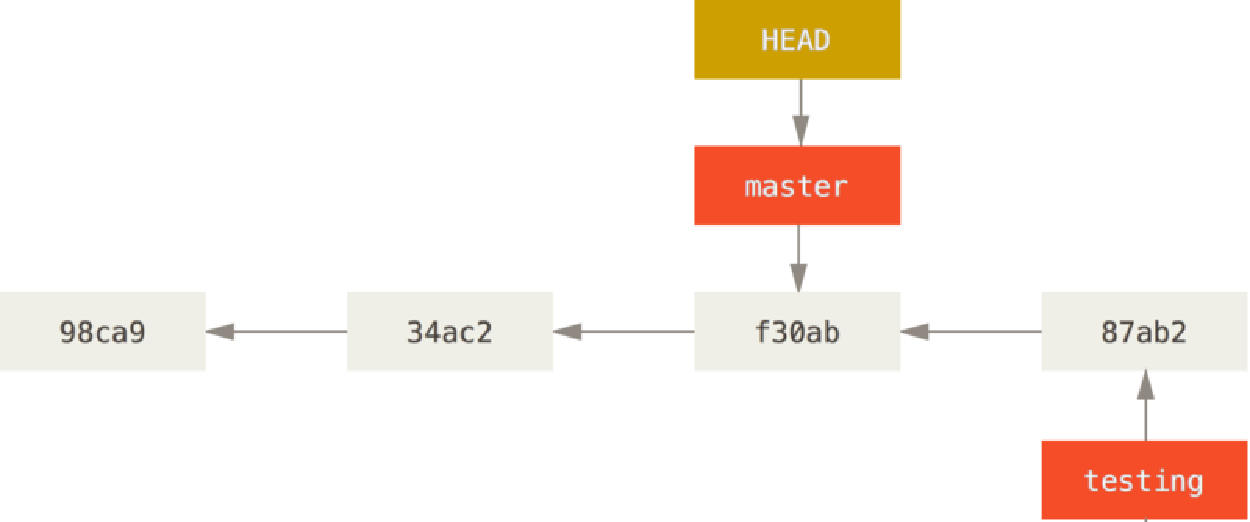
\includegraphics[width=0.9\textwidth]{branching-git.pdf}}
\end{frame}

\begin{frame} \frametitle{Особенности Git}
  \begin{itemize}
  \item Снимки, а не различия
  \item Почти все операции выполняются локально
  \item Целостность Git
  \item Git только добавляет данные
  \item Три состояния
  \end{itemize}
\end{frame}

\lecturenotes

Снимки, а не различия
Основное отличие Git’а от любой другой СКВ, это подход Git’а к работе со своими данными. Концептуально, большинство других систем хранят информацию в виде списка изменений в файлах. Эти системы представляют информацию в виде набора файлов и изменений, сделанных в каждом файле, по времени. 
Git не хранит и не обрабатывает данные таким способом. Вместо этого, подход Git’а к хранению данных больше похож на набор снимков миниатюрной файловой системы. Каждый раз, когда вы делаете коммит, то есть сохраняете состояние своего проекта в Git’е, система запоминает, как выглядит каждый файл в этот момент, и сохраняет ссылку на этот снимок. Для увеличения эффективности, если файлы не были изменены, Git не запоминает эти файлы вновь, а только создаёт ссылку на предыдущую версию идентичного файла, который уже сохранён. Git представляет свои данные как, скажем, поток снимков.

Почти все операции выполняются локально
Для работы большинства операций в Git достаточно локальных файлов и ресурсов — в основном, системе не нужна никакая информация с других компьютеров в вашей сети. Если вы привыкли к ЦСКВ, где большинство операций имеют задержку из-за работы с сетью, то этот аспект Git’а заставит вас думать, что боги скорости наделили Git несказанной мощью. Так как вся история проекта хранится прямо на вашем локальном диске, большинство операций кажутся чуть ли не мгновенными.

Это также означает, что есть лишь небольшое количество действий, которые вы не сможете выполнить, если вы находитесь оффлайн или не имеете доступа к VPN в данный момент. Если вы в самолёте или в поезде и хотите немного поработать, вы сможете создавать коммиты без каких-либо проблем: когда будет возможность подключиться к сети, все изменения можно будет синхронизировать.

Целостность Git
В Git’е для всего вычисляется хеш-сумма, и только потом происходит сохранение. В дальнейшем обращение к сохранённым объектам происходит по этой хеш-сумме. Это значит, что невозможно изменить содержимое файла или директории так, чтобы Git не узнал об этом. Данная функциональность встроена в Git на низком уровне и является неотъемлемой частью его философии. Вы не потеряете информацию во время её передачи и не получите повреждённый файл без ведома Git.

Git только добавляет данные
Когда вы производите какие-либо действия в Git, практически все из них только добавляют новые данные в базу Git. Очень сложно заставить систему удалить данные либо сделать что-то, что нельзя впоследствии отменить. Как и в любой другой СКВ, вы можете потерять или испортить свои изменения, пока они не закоммичены, но после того, как вы закоммитите снимок в Git, будет очень сложно что-либо потерять, особенно, если вы регулярно синхронизируете свою базу с другим репозиторием

Три состояния
Git имеет три основных состояния, в которых могут находиться файлы: зафиксированном (committed), изменённом (modified) и подготовленном (staged). “Зафиксированный” значит, что файл уже сохранён в локальной базе. К изменённым относятся файлы, которые поменялись, но ещё не были зафиксированы. Подготовленные файлы — это изменённые файлы, отмеченные для включения в следующий коммит~\cite[с.~8-10]{ProGit}.

\begin{frame} \frametitle{Три состояния проекта в Git}
  \centerline{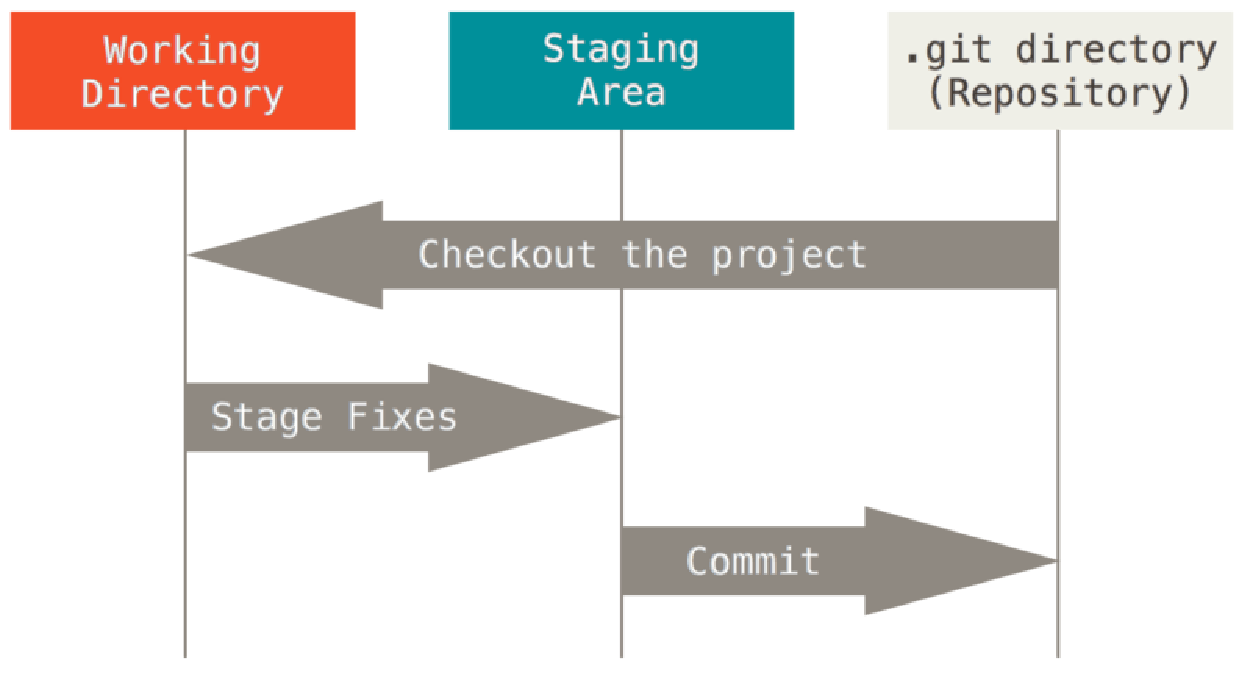
\includegraphics[width=0.9\textwidth]{GitSections.pdf}}
\end{frame}

\lecturenotes

У проекта Git есть три основные секции: Git-директория (Git directory), рабочая директория (working directory) и область подготовленных файлов (staging area).

Git-директория --- это то место, где Git хранит метаданные и базу объектов проекта. Это самая важная часть Git, и это та часть, которая копируется при клонировании репозитория с другого компьютера.
Рабочая директория является снимком версии проекта. Файлы распаковываются из сжатой базы данных в Git-директории и располагаются на диске, для того чтобы их можно было изменять и использовать.
Область подготовленных файлов — это файл, располагающийся в Git-директории, в нём содержится информация о том, какие изменения попадут в следующий коммит. Эту область ещё называют “индекс”, однако stage-область так же общепринятое название~\cite[с.~11]{ProGit}.

\begin{frame} \frametitle{Недостатки Git}
  
  \begin{itemize}
  \item Отсутствие сквозной нумерации коммитов монотонно непрерывно возрастающими целыми числами
  \item Использование для идентификации ревизий хешей SHA1 не всегда бывает удобно
  \item Большие накладные расходы при работе с проектами, в которых делаются многочисленные несвязанные между собой изменения файлов
  \item Отсутствие отдельной команды переименования/перемещения файла, которая отображалась бы в истории как соответствующее единое действие
  \item Низкоуровневый и довольно сложный интерфейс, что увеличивет порог входа в данную VCS
  \end{itemize}
\end{frame}

\lecturenotes

Отсутствие сквозной нумерации коммитов монотонно непрерывно возрастающими целыми числами. Во многих проектах используется автоматическое получение номера этой версии (например, командой svnversion), построение .H файла на основе этого числа, и далее его использование при создании штампа версии исполняемого файла, некоторых вшитых в него строк и так далее.

Некоторое неудобство для пользователей, переходящих с других VCS. Команды git, ориентированные на наборы изменений, а не на файлы, могут вызвать недоумение у пользователей, привыкших к файл-ориентированным VCS, таким как SVN. Например, команда «add», которая в большинстве систем управления версиями производит добавление файла к проекту, в git подготавливает к фиксации сделанные в файлах изменения. При этом сохраняется не патч, описывающий изменения, а новая версия целевого файла.

Использование для идентификации ревизий хешей SHA1, что приводит к необходимости оперировать длинными строками вместо коротких номеров версий, как во многих других системах (хотя в командах допускается использование неполных хеш-строк).

Большие накладные расходы при работе с проектами, в которых делаются многочисленные несвязанные между собой изменения файлов. При работе в таком режиме размеры наборов изменений становятся достаточно велики и происходит быстрый рост объёма репозиториев.

Отсутствие отдельной команды переименования/перемещения файла, которая отображалась бы в истории как соответствующее единое действие. Существующий скрипт git mv фактически выполняет переименование, копирование файла и удаление его на старом месте, что требует специального анализа для определения, что в действительности файл был просто перенесён (этот анализ выполняется автоматически командами просмотра истории). Однако, учитывая тот факт, что наличие специальной команды для переименования/перемещения файлов технически не вынуждает пользователя использовать именно её (и, как следствие, в этом случае возможны разрывы в истории), поведение git может считаться преимуществом.

Система работает только с файлами и их содержимым, и не отслеживает пустые каталоги~\cite{GitWikipedia}.

\subsection{Mercurial}

\begin{frame} \frametitle{Mercurial}
  \begin{block}{}
    \alert{Mercurial, он же Hg (от обозначения химического элемента ртути)} --- кроссплатформенная распределённая система управления версиями, разработанная для эффективной работы с очень большими репозиториями кода
  \end{block}
\end{frame}

\begin{frame} \frametitle{Ревизии в Mercurial}
  \begin{itemize}
  \item Ревизия --- это сущность, описывающая изменения в каких-либо файлах. Эта сущность хранит информацию о своём авторе, времени создания, изменениях в файлах и о родительских ревизиях
  \item Ревизия идентифицирует не только себя, но и всю свою историю
  \item Номер ревизии представляет собой целое число, отражающее порядок, в котором наборы изменений были добавлены в хранилище
  \item Ревизии организовывают ориентированный ациклический граф
  \item Существуют две специальные ревизии: null (ревизия-родитель) и tip (самая последняя ревизия)
  \end{itemize}
\end{frame}

\lecturenotes

Ревизия (changeset) - это сущность, описывающая изменения в каких-либо файлах. Эта сущность хранит информацию о своём авторе, времени создания, изменениях в файлах и о родительских ревизиях (которых может быть одна в случае обычной ревизии и две в случае слияния). Кстати, подсчёт 40-цифрового 16-ричного sha1-хеша, которым идентифицируется ревизия, учитывает все эти значения - таким образом каждая ревизия идентифицирует не только себя, но и всю свою историю.

Эти ревизии (благодаря наличию у себя родителей) организовывают ориентированный ациклический граф (от ревизии 0 и до существующих голов), который может разветвиться в любом месте.

Головы - это ревизии, у которых (ещё) нет детей, конечные точки графа.

При этом существуют две специальные ревизии - null (ревизия-родитель самой первой ревизии под номером 0) и tip (самая последняя ревизия, в случае наличия нескольких голов выбирается в зависимости от обстоятельств)~\cite{MercurialSolovyov}.

\begin{frame} \frametitle{Ветвление в Mercurial}
  \begin{itemize}
  \item Ветка представляет собой связанную последовательность ревизий
  \item Название ветки стоит из хэш-суммы и порядкового номера
  \item Ветка могут быть анонимными  и именованными
  \item Можно создать ветку путем создания локальной копии всего репозитория, но такой способ довольно медленный
  \end{itemize}
\end{frame}

\lecturenotes

Анонимное ветвление

На самом деле, создание ветви при работе с Mercurial не является чем-то из ряда вон выходящим, для распределенной модели контроля версий это стандартная операция, и поэтому может быть произведена крайне просто, фактически, простым коммитом. То есть мы должны привести рабочую копию в состояние отличное от "вершины" (tip), внести изменения и выполнить коммит. Ничего больше. 

 Локальность производимых ветвлений - это главное, коренное, отличие от централизованных систем контроля версий, в том числе от Subversion. Никто не увидит вашей ветви до тех пор пока вы не синхронизируете свой репозиторий с удаленным (обычно командой push). С другой стороны выполнение pull приведет к появлению в вашем репозитории всех ветвей, имеющихся в удаленном.

Преимущества
Основным преимуществом этого способа является крайняя простота. Не нужно ничего придумывать, выполнять сложных операций, оповещать других участников команды - просто апдейт и коммит.

Недостатки
Недостатки вытекают из анонимности ветви. Фактически, понять, что у вас есть ветвь разработки, исходя из вывода стандартных операций Mercurial, затруднительно. Особенно после 2-3 месяцев активной работы с репозиторием, когда количество таких мелких ветвлений приближается к сотне. Соответственно вам придется писать информативные подписи к коммитам, если анонимные ветви предполагается использовать в дальнейшем. Для переключения между ветвями разработки вам придется использовать номер ревизии, который, как известно, простой хэш - очень удобен для машины, но крайне неудобен для человека.

Таким образом, анонимные ветви - это отличный механизм для внесения быстрых (по количеству ревизий) исправлений, логически сильно связанных с направлением основной ветви разработки, то есть для организации ветвления на 2-3 ревизии с последующим слиянием с основной ветвью. Для организации больших ветвей, логически необходимых для разделения направлений разработки следует использовать именованные ветви.

Именованное ветвление

Вполне естественно, что в Mercurial предусмотрен способ создания ветвей разработки с некоторыми именами, задаваемыми пользователем. Для организации подобных ветвлений предназначена команда hg branch. С помощью этой команды версия, находящаяся в локальной копии помечается ветвью с новым именем, при этом сама ветвь будет создана только после того, как вы выполните коммит

Отмечу лишь один очень важный факт - ветвление произведено в вашем локальном репозитории, и вы можете работать с ним так, как вам угодно, при этом вы не боитесь поломать чужой код своим коммитом, или вызвать у тимлида приступ головной боли своими ветвлениями. Вот именно так концепция распределенной системы контроля версий позволяет решить стандартные болячки централизованных систем.

Преимущества
Итак именованное ветвление лишь немногим сложнее анонимного, однако позволяет организовать работу над сложным проектом с несколькими направлениями разработки наиболее эффективным образом. Имя ветви является метаданными каждой ревизии, что позволяет корректно отслеживать изменения, произошедшие в проекте. Хотя принципиальных отличий от анонимных ветвей, на самом деле, нет.

Недостатки
К недостаткам, в некоторой степени, можно отнести синдром разрастания ветвей. То есть, если вы будете использовать именованные ветви при каждой необходимости отпочковаться от основной, вывод команды hg branches будет просто гиганским через некоторое время. Хотя ветви можно закрывать при коммитах (опция --close-branch), не стоит делать именованные ветви там где они не нужны.
Ветвление в клонах репозитория

Последний способ организации ветвления о котором я расскажу - ветвление в клонах. На самом деле способ очевиден, и вытекает из третьей части этого цикла. Ничто не мешает пользователю лично создать клон репозитория и в нем вести отдельную ветвь разработки. Таким образом, для каждой ветви потребуется отдельный репозиторий. Безусловно модель распределенной системы контроля версий Mercurial позволяет подобную трактовку ветвления разработки, однако рассмотрим аспекты подобного подхода:

Преимущества
Немного более безопаснее чем при других способах. На самом деле в данном случае способ выстрелить себе в ногу только один - запушить что нибудь этакое в удаленный репозиторий, тогда как при локальном ветвлении способов выстрелить себе в ногу немного больше.

Недостатки
На мой взгляд недостатки перевешивают все преимущества. Самый главный недостаток - при каждом клонировании вам придется вытягивать весь репозиторий, то есть, если вам захотелось получить доступ к некоторой ветви вам придется вытянуть весь репозиторий относящийся к этой ветви, и так для каждой. Второй недостаток - бекапить вам придется не один репозиторий, а несколько. Что не логично. ~\cite{MercurialBrainIt}.

\begin{frame} \frametitle{Пример ветвления}
  \centerline{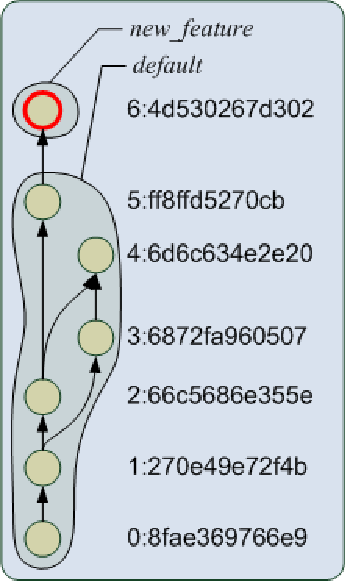
\includegraphics[width=0.3\textwidth]{branching-mercurial.pdf}}
\end{frame}

\begin{frame} \frametitle{Особенности Mercurial}
  
  \begin{itemize}
  \item Прост в изучении и использовании
  \item Легковесный
  \item Может использоваться в проектах любого масштаба
  \item Легко настраивается под конкретные нужды
  \end{itemize}
\end{frame}

\lecturenotes

Mercurial обладает уникальным набором свойств, позволяющим выбрать его в качестве наиболее подходящей системы контроля версий: Прост в изучении и использовании, Легковесный, Превосходно масштабируется, Легко настраивается под конкретные нужды.

Mercurial предоставляет единообразную и последовательную систему команд и функций, что позволяет руководствоваться небольшим набором общих правил вместо того, чтобы учить массу исключений.

В небольших проектах вы можете начать работу с Mercurial в считанные минуты. Создание новых веток и изменений, распространение изменений (как локально, так и по сети), операции с историей и статусом — всё это работает быстро. Mercurial старается быть незаметным и не путаться под вашими ногами, не требует от вас больших умственных усилий и совершает свои операции невероятно быстро.

Mercurial применяется не только в маленьких проектах, его используют и в проектах с сотнями и тысячами разработчиков, проектах, которые содержат десятки тысяч файлов и сотни мегабайт исходного кода.

Если вам не хватает базовой функциональности Mercurial, то её легко расширить. Mercurial хорошо подходит для задач скриптинга, его понятное устройство и реализация на языке Python позволяет легко добавлять новые возможности в виде расширений. Существует большое количество популярных и полезных расширений, охватывающих спектр задач от помощи в нахождении ошибок до улучшения производительности~\cite[с.~6--7]{MercurialOReilly}.

\begin{frame} \frametitle{Возможности Mercurial}
  
  \begin{itemize}
  \item Обладает превосходной производительностью
  \item Репозиторий Mercurial не требует операций по техническому обслуживанию
  \item Используются стандартные протоколы для обмена данными между репозиториями (http(s), ssh)
  \item Возможен импорт истории изменений из репозитория Subversion или Git
  \end{itemize}
\end{frame}

\lecturenotes

Git очень быстр. В некоторых случаях он быстрее, чем Mercurial (по крайней мере под Linux), а в других быстрее оказывается Mercurial. Однако под Windows как производительность, так и общий уровень поддержки, во время написания этой книги у Git гораздо хуже, чем у Mercurial.

В то время как репозиторий Mercurial не требует операций по техническому обслуживанию, репозиторий Git требует частых ручных «перепаковок» собственных метаданных. Если этого не делать, производительность начинает падать, наряду с увеличением объёма занимаемого дискового пространства. Дисковый массив сервера, содержащего несколько Git репозиториев, по отношению к которым не выполняется строгое правило частой «перепаковки», рано или поздно забивается под завязку, в результате чего процесс ежедневного резервного копирования легко может занимать более 24 часов. 

Использование абсолютно стандартных протоколов для обмена данными между репозиториями: http (и https), ssh или, на худой конец, аттачами в email.
При этом никаких усилий или отдельных демонов не требуется. ssh работает без всякой настройки, а http-часть идёт в комплекте и требует веб-сервера, могущего cgi/fastcgi/wsgi (на выбор). Протоколы работы по ним очень похожи - локальный и удалённый меркуриалы обмениваются bundle’ами, сжатыми файлами с группой ревизий.

Mercurial может импортировать историю изменений из репозитория Subversion. Возможен и обратный процесс. Это делает возможным прощупать почву и использовать Mercurial и Subversion одновременно, прежде чем решить, осуществлять переход или нет. Преобразование истории — пошаговый процесс, так что вы можете осуществить начальное преобразование, а потом вносить новые изменения.
Mercurial предоставляет возможность импорта истории версий из репозитория Git~\cite[с.~7--9]{MercurialOReilly}.

\begin{frame} \frametitle{Недостатки Mercurial}
  
  \begin{itemize}
  \item Невозможно размещать и раздельно использовать несколько проектов в одном репозитории
  \item Нет возможности слияния двух родительских веток
  \item Mercurial использует систему плагинов, а не поддержку скриптов
  \end{itemize}
\end{frame}

\lecturenotes

Некоторые ожидают что с помощью hg можно размещать и раздельно использовать несколько проектов в одном репозитории. В действительности, это не то, ради чего hg был создан. В частности, это означает, что вы не можете получить из репозитория только один каталог~\cite{MercurialWiki}.

Один из существенных недостатков Mercurial заключается в том, что в отличии от Git в ней нельзя объединить две родительские ветки, так как Mercurial использует систему плагинов, а не поддержку скриптов~\cite{MercurialTD}.

\section{Коллективная разработка с использованием систем контроля версий}

\begin{frame} \frametitle{Использование веток}
  \begin{itemize}
  \item Стволовая ветвь (trunk) --- это основное направление разработки. Большая часть ветвлений и слияний происходит с ней. Стволовая ветвь создаётся один раз при создании нового хранилища и существует на протяжении всего жизненного цикла проекта
  \item Перед выпуском очередной версии релиза программного обеспечения обычно создаётся релизная ветвь (release branch), изменения в которой строго регламентированы. В основном в неё попадают исправления серьёзных ошибок, обнаруженных при подготовке версии. Все остальные изменения вносятся в стволовую ветвь
  \item Функциональная ветвь (functional branch) создаётся для выполнения серии дестабилизирующих изменений без влияния на стволовую ветвь
  \end{itemize}
\end{frame}

\lecturenotes

Использование ветвей

Существует ряд приёмов ветвления, широко применяемых прежде всего при разработке программного обеспечения.
Стволовая ветвь

История изменений каждого документа в хранилище представляет собой древовидную структуру. Стволовая ветвь (англ. trunk) это основное направление разработки. Большая часть ветвлений и слияний происходит с ней. Стволовая ветвь создаётся один раз при создании нового хранилища и существует на протяжении всего жизненного цикла проекта. Все остальные ветви создаются для определённых целей и различаются по своему назначению.

Релизная ветвь
Перед выпуском очередной версии релиза программного обеспечения недопустимо вносить потенциально дестабилизирующие изменения в исходный код. Поэтому перед выпуском обычно создаётся релизная ветвь (англ. release branch или англ. tag), изменения в которой строго регламентированы. В основном в неё попадают исправления серьёзных ошибок, обнаруженных при подготовке версии. Все остальные изменения вносятся в стволовую ветвь. Таким образом, стабильность кода на релизной ветви не нарушается, и релиз выпускается из кода этой ветви. В дальнейшем можно путём слияния перенести исправления, сделанные на релизной ветви, и на стволовую ветвь. Как правило, релизная ветвь после выпуска версии не удаляется. Она может понадобиться для воспроизведения состояния проекта на момент выпуска.

Функциональная ветвь
Функциональная ветвь (англ. functional branch) создаётся для выполнения серии дестабилизирующих изменений без влияния на стволовую ветвь. Например, нужно добавить в код новую функциональность, но изменения настолько сложны, что их нельзя выполнить за одну фиксацию. Либо требуется участие нескольких человек. В этом случае создаётся ветвь, в которую вносятся дестабилизирующие изменения. При этом код на ветви может продолжительное время пребывать в нестабильном состоянии. Когда изменения выполнены и код приведён в стабильное состояние, производится слияние изменений в стволовую ветвь. Таким образом, на стволовой ветви изменения, сделанные на функциональной ветви, выглядят как одна фиксация (фиксация, которой выполнено слияние), при этом нестабильных промежуточных состояний на стволовой ветви нет. Они есть только на функциональной ветви, где их можно посмотреть при необходимости. После слияния жизненный цикл функциональной ветви закончен, её можно удалить~\cite{Branching}.

\begin{frame} \frametitle{Фиксация изменений}
  \begin{itemize}
  \item Используется описательное сообщение для фиксации изменений, чтобы в дальнейшем можно было понять, о чём оно
  \item Одно изменение представляет из себя одну логическую единицу, с определённой целью
  \end{itemize}
\end{frame}

\begin{frame} \frametitle{Конкурентное редактирование}
  \begin{itemize}
  \item Несколько человек могут редактировать один и тот же файл одновременно
  \item Система управления версиями автоматически объединяет их изменения
  \item Если два человека отредактируют одни и те же строки кода, система управления версиями предложит им объединить две строки вручную
  \end{itemize}
\end{frame}

\lecturenotes

Эта модель позволяет двум людям одновременно редактировать один и тот же файл. Система контроля версий автоматически объединяет свои изменения - ничто не перезаписывается случайно. Если два человека отредактируют одни и те же строки кода, система управления версиями предложит им объединить две строки вручную. Автоматическое слияние может показаться рискованным. Они были бы рискованными, если бы не непрерывная интеграция и автоматическая сборка. Непрерывная интеграция уменьшает объем слияний до уровня управления, а сборка с ее полным набором тестов подтверждает, что слияния работают правильно~\cite[170-171]{AgileDevelopment}.

\begin{frame} \frametitle{Разрешение конфликтов}
Конфликты возникают если
  \begin{itemize}
  \item один и тот же файл был изменен как в локальном, так и в удаленном репозитории, и
  \item автоматическое слияние изменений не произошло, поскольку изменения находятся в одном и том же месте файла
  \end{itemize}
Разрешение конфликтов
  \begin{itemize}
  \item Файлы, содержащие исходный код, необходимо отредактировать с учетом или без учета внесенных обеими сторонами изменений
  \item Далее делается коммит, фиксирующий слияние
  \end{itemize}
\end{frame}

\lecturenotes

Разрешение конфликтов
Общие сведения

Конфликты синхронизации происходят, если выполнены оба условия

    один и тот же файл был изменен как в локальном, так и в удаленном репозитории, и

    автоматическое слияние изменений не произошло, поскольку изменения находятся в одном и том же месте файла.

Типичные случаи:

    бинарный файл (текстура, blend-файл) независимо изменен двумя участниками разработки

    в текстовой файл в одной и той же строке были внесены разные изменения

    один участник разработки изменил файл, а другой - переместил его и т.п.

Хотя конфликты синхронизации - нормальное явление, слишком частое их возникновение замедляет работу. Рекомендуется ставить коллег в известность о начале работ с общими бинарными файлами, а также чаще проводить синхронизацию.

Порядок действий
Не рекомендуется производить какие-либо действия с файлами (изменять, удалять), пока репозиторий находится в конфликтном состоянии.
Дальнейший порядок действий различен для бинарных и текстовых файлов.

Бинарные файлы
На данном этапе конфликтующие бинарные файлы находятся в том состоянии, в котором они находились в локальном репозитории до попытки синхронизации. Файлы полностью функциональны (например, открываются графическими редакторами).
В случае конфликта бинарных файлов необходимо выяснить с коллегами или самостоятельно, какую из версий оставить, а какую отбросить. Выбор осуществляется командой git checkout.
В итоге необходимо остановиться на нужной версии файла. При угрозе потери работы можно сохранить отбрасываемую версию файла вне репозитория.

Текстовые файлы
На данном этапе в конфликтующие текстовые файлы Git’ом вносятся как локальные, так и удаленные изменения одновременно, в особом формате. Такие текстовые файлы как правило, не работоспособны.

В случае конфликта текстовых файлов можно поступить следующим образом. Файлы, содержащие исходный код, необходимо отредактировать с учетом или без учета внесенных обеими сторонами изменений. В то же время экспортированные текстовые файлы сцен (заканчивающиеся на .json) проще повторно экспортировать.

Корректирующий коммит
Выполнить коммит, комментарий рекомендуется оставить предложенный по умолчанию.
Конфликты разрешены, изменения из удаленного репозитория успешно применены в локальном репозитории. Теперь изменения в локальном репозитории, - включающие только что разрешенный конфликт, - можно загрузить в удаленный репозиторий командой git push~\cite{Blend4web}.

\begin{frame} \frametitle{Строгое версионирование}
  \begin{itemize}
  \item С помощью систем управления версиями все версии проекта автоматически сохраняются в упорядоченном виде
  \item В любой момент можно просмотреть предыдущие версии, увидеть различия с текущей версией
  \end{itemize}
\end{frame}

\lecturenotes

Строгое версионирование

Сохранение версии вашего проекта после внесения изменений является важной привычкой. Но без VCS это становится утомительным и запутывающим очень быстро:

    Сколько вы сохраняете? Только измененные файлы или полный проект? В первом случае вам будет сложно просмотреть весь проект в любой момент времени - в последнем случае у вас будет огромное количество ненужных данных, лежащих на вашем жестком диске.
    Как вы называете эти версии? Если вы очень организованный человек, вы можете придерживаться действительно понятной схемы именования (если вы довольны «acme-inc-redesign-2013-11-12-v23»). Однако, как только дело доходит до вариантов (скажем, вам нужно подготовить одну версию с областью заголовка и без нее), скорее всего, вы в конечном итоге потеряете трек.
    Однако самый важный вопрос, вероятно, следующий: откуда вы знаете, что в этих версиях отличается? Очень немногие люди на самом деле тратят время на тщательное оформление каждого важного изменения и включают это в файл README в папке проекта.

Система управления версиями признает, что существует только один проект. Поэтому на вашем диске есть только одна версия, над которой вы сейчас работаете. Все остальное - все прошлые версии и варианты - аккуратно собраны внутри VCS. Когда вам это нужно, вы можете запросить любую версию в любое время, и у вас будет мгновенный снимок всего проекта прямо под рукой~\cite{GitTower}.

\begin{frame} \frametitle{Возвращение к предыдущему коду}
  \begin{itemize}
  \item Один из сильнейших возможностей систем контроля версий --- это возможность вернуть всю кодовую базу к определённой точки в прошлом
  \item Идя от старых версий к новым можно найти место, в котором была совершена ошибка
  \item Путешествие во времени также полезно для воспроизведения ошибок. Если кто-то сообщает об ошибке, и не получается воспроизвести ее, можно использовать ту же версию кода, в которой была обнаружено ошибка
  \end{itemize}
\end{frame}

\lecturenotes

Одним из самых мощных способов использования системы управления версиями является способность вернуться во времени. Вы можете обновить вашу песочницу со всеми файлами с определенной точки в прошлом.
Это позволяет использовать отладку diff. Когда вы обнаружите сложную ошибку, которую вы не можете нормально отлаживать, вернитесь вовремя к старой версии кода, когда ошибка не существует. Затем идите вперед и назад, пока не выделите точную регистрацию, в которой введена ошибка. Вы можете просмотреть изменения только в этой регистрации, чтобы узнать причину ошибки. При непрерывной интеграции количество изменений будет небольшим.

Путешествие во времени также полезно для воспроизведения ошибок. Если кто-то сообщает об ошибке, и вы не можете воспроизвести ее, попробуйте использовать ту же версию кода, которую использует репортер. Если вы можете воспроизвести поведение в старой версии, но не в текущей версии, особенно с модульным тестом, вы можете быть уверены, что ошибка будет и останется фиксированной~\cite[171]{AgileDevelopment}.


\begin{frame} \frametitle{Дополнительные возможности}
  \begin{itemize}
  \item Система контроля версий может выступать в качестве инструмента резервного копирования, т.к. каждый член команды  имеет полномасштабную версию проекта
  \item Понимание происходящего в проекте, за счёт сохранения описаний каждого изменения
  \end{itemize}
\end{frame}

\lecturenotes

Резервное копирование
Побочным эффектом использования распределенного VCS, такого как Git, является то, что он может выступать в качестве резервной копии; каждый член команды имеет полномасштабную версию проекта на своем диске, включая полную историю проекта. Если ваш любимый центральный сервер сломается (и ваши резервные диски не работают), все, что вам нужно для восстановления, является одним из локальных хранилищ Git вашего товарища по команде.

Понимание того, что произошло

Каждый раз, когда вы сохраняете новую версию своего проекта, ваш VCS требует от вас краткого описания того, что было изменено. Кроме того (если это код / текстовый файл), вы можете увидеть, что именно было изменено в содержимом файла. Это поможет вам понять, как ваш проект развивался между версиями~\cite[171]{AgileDevelopment}.


\begin{thebibliography}{99}
\bibitem{Atlassian} \href{https://www.atlassian.com/git/tutorials/what-is-version-control}{What is version control | Atlassian Git Tutorial}
\bibitem{ProGit} Scott Chacon Pro Git 1st Edition. Apress, 2009
\bibitem{VSwithSVN} 	Brian Fitzpatrick, C. Pilato, Ben Collins-Sussman Version Control with Subversion. O'Reilly Media, 2009
\bibitem{SVNMotu} \href{http://henry-motu.org.ua/2010/10/02/subversion-svobodnaja-sistema-upravkenija-versijam/}{Subversion --- свободная система управления версиями | Henry Motu}
\bibitem{SVNWikipedia} \href{https://ru.wikipedia.org/wiki/Subversion}{Subversion --- Википедия}
\bibitem{GitWikipedia} \href{https://ru.wikipedia.org/wiki/Git}{Git --- Википедия}
\bibitem{MercurialOReilly} Bryan O'Sullivan Mercurial: The Definitive Guide. O'Reilly Media, 2009
\bibitem{MercurialSolovyov} \href{https://solovyov.net/blog/2008/mercurial-basics/}{solovyov.net: Mercurial: основы}
\bibitem{MercurialBrainIt} \href{http://brain-it.blogspot.ru/2010/01/mercurial-4.html}{Brain IT!: Введение в Mercurial. Часть 4. Способы организации ветвей}
\bibitem{MercurialWiki} \href{https://www.mercurial-scm.org/wiki/RussianUnderstandingMercurial}{Understanding Mercurial --- Mercurial}
\bibitem{MercurialTD} \href{https://biz30.timedoctor.com/ru/cистема-контроля-версий/}{Система контроля версий (cvs) 2017 - Сравниваем: Git, SVN, Mercurial}
\bibitem{Branching} \href{https://ru.wikipedia.org/wiki/Ветвь_(управление_версиями)}{Ветвь (управление версиями) — Википедия}
\bibitem{Blend4web} \href{https://www.blend4web.com/doc/ru/git_short_manual.html}{Работа в команде с использованием Git. Руководство пользователя Blend4Web 17.10}
\bibitem{AgileDevelopment} James Shore, Shane Warden The Art of Agile Development. O'Reilly, 2008
\bibitem{GitTower} \href{https://www.git-tower.com/learn/git/ebook/en/command-line/basics/why-use-version-control}{Why Use Version Control?}
\end{thebibliography}

\end{document}

%%% Local Variables: 
%%% mode: TeX-pdf
%%% TeX-master: t
%%% End: 
